\documentclass[12pt,a4paper]{report}
\usepackage{geometry}
\geometry{top=14mm, bottom=15mm}
\usepackage[english]{babel}
\usepackage[utf8]{inputenc}
\usepackage{fancyhdr}
\usepackage{listings}
\usepackage{graphics, graphicx}
\usepackage{graphics, graphicx}
\pagestyle{fancy}
\fancyhf{}
%\rhead{}
%\lhead{}
\fancyfoot[LE,LO]{Data Analytics}
\fancyfoot[RE,RO]{Mini Project - 1}
\renewcommand{\footrulewidth}{1pt}
 \medskip
 \author{Abhijeet Singh Panwar (ID : 201351005)}
\title{Data Analytics\\ Mini Project - 1}

\date{\parbox{\linewidth}{\centering%
  \today\endgraf\bigskip
  Instructor : \endgraf\medskip
  Prof. Bhargab Chattopadhyay\endgraf\bigskip
  Indian Institute of Information Technology, Vadodara}}
\begin{document}
\maketitle
\newpage
\section{Overview for simulating the experment}
\textbf{Given:}\\
\begin{itemize}
\item A program is divided into 3 blocks \& each block runs in parallel manner.
\item Average time taken by each block = 5 minutes (independent of other blocks).
\item Each block takes an exponential amount of time.
\item Program completes, when all blocks get completed.
\end{itemize}

\textbf{Algorithm}
\begin{itemize}
\item From above given conditions, it is evident that time required for program to get competely compiled = Execution time of slowest thread.
\item Therefore, \textbf{X}(time taken by program for compilation) = Maximum(value of $x_1$, $x_2$, $x_3$, name of each thread as denoted in below R code).
\item Finally, E[X] = average of all values of X.
\end{itemize}

\section{Section 2}
\textbf{Part A \& B}
\\
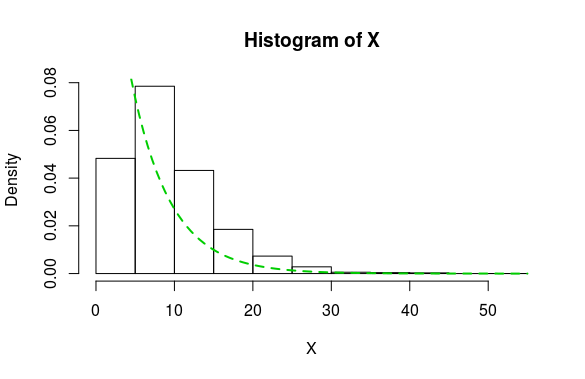
\includegraphics[scale=0.8]{hist2.png}
\\
The image represents the histogram generated from simulated values and the green dotted line shows the density function for exponential distribution.
\\\\
\textbf{Part C}
\\\\
Using, the fact that:\\\\
E[X] = 1/$\lambda$ = 5 , Var[X] = 1/${\lambda}^2$ = 25\\\\
\& Var[X] = $E[X^2] - {E[X]}^2$\\\\
Therefore, $E[X^2]$(theoritical) = 50\\\\
But, $E[X^2]$(experimental) = 116.66\\\\
Difference = 66.66\\\\
\textbf{Part D}\\\\
${E[X^2]}_1$(experimental) = 117.12 \& Difference = 67.12\\
${E[X^2]}_2$(experimental) = 116.15 \& Difference = 66.15\\
${E[X^2]}_3$(experimental) = 117.14 \& Difference = 67.14\\
${E[X^2]}_4$(experimental) = 118.64 \& Difference = 68.64\\
${E[X^2]}_5$(experimental) = 120.29 \& Difference = 70.29\\
\\
\textbf{Part E}
\\\\
\textbf{For 1,000 replications:}\\

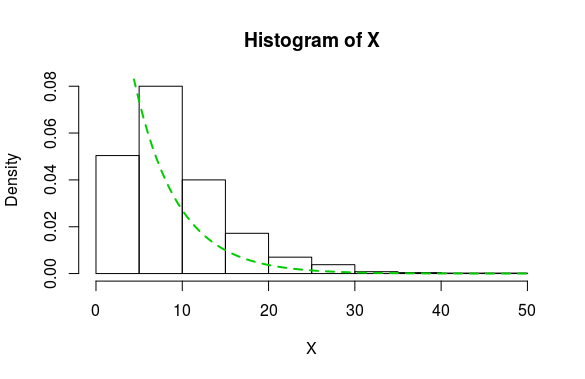
\includegraphics[scale=0.8]{1.png}\\
E[X] = 9.27\\
E[$X^2$] = 123.47\\

\textbf{For 1,00,000 replications:}\\

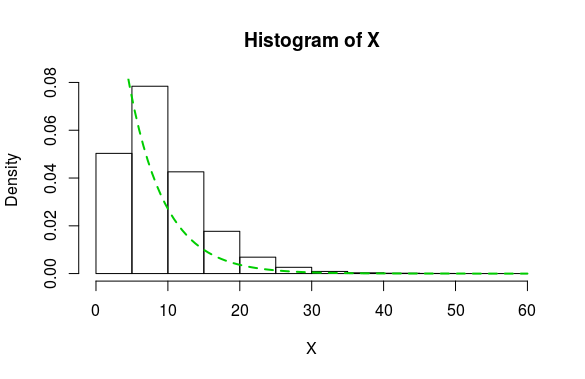
\includegraphics[scale=0.8]{2.png}\\
E[X] = 9.19\\
E[$X^2$] = 118.74\\
\\
\textbf{Inference:}\\

Between 1,000 and 1,00,000 simulations, there is a slight difference in E[X] and a significant difference is observed in E[$X^2$]. This is because as number of simulations increases E[X] \& E[$X^2$] gets more closer to the theoritical E[X] \& E[$X^2$].

\section{R-Code}
For Part A \& Part B\\
\begin{lstlisting}
X=c() #initializing a column vector of total time for 
		#complete compilation of program
X2=c()#square of total time

for (i in 1:10000) #for each i
{  x1 = rexp(1,rate=0.2) # generate random x1, x2, x3
x2 = rexp(1,rate=0.2)    # for exponential distribution, 
			#for rate = 0.2
x3 = rexp(1,rate=0.2)
m=max(x1,x2,x3)
X=c(X,m) #appending the maximum time taken by a thread 
		#into compilation time vector
X2 = c(X2,m^2)
}
hist(X,prob=TRUE) #here curve in plotting is used to 
				#superimpose two graphs
curve(dexp(x,rate=0.2), col=3, lty=2,lwd=2,add=TRUE)
mean(X) #Expectatio of X
mean(X2)#Expectation of X^2
\end{lstlisting}

\end{document}